\section{Evaluation} \label{sec:evaluation}

We evaluate our system on the multi-class, multi-label detection task as previously described.
Each detection episode takes an image and outputs detections with associated times, based on the order of actions taken.
We evaluate on a popular detection challenge task: the PASCAL VOC 2007 dataset \cite{pascal-voc-2010}, which exhibits only a rather modest amount of class co-occurrence: the ``person'' class is highly likely to occur, and less than $10\%$ of the images have more than two classes.

We learn weights on the training and validation sets, and run our policy on all images in the testing set.
The final evaluation pools all detections up to a certain time, and computes their multi-class AP per image, averaging over all images.
This is done for different times to plot the AP vs. Time curve over the whole dataset.
Our method of averaging per-image performance follows \cite{Desai2009}.

For the detector actions, we use one-vs-all cascaded deformable part-model detectors on a HOG featurization of the image \cite{Felzenszwalb2010b}, with associated linear classification of the detections.
There are $20$ classes in the PASCAL challenge task, so there are $20$ detector actions.
Running a detector on a PASCAL image takes about $1$ second.

We test three different settings of the start and deadline times.
In the first one, the start time is immediate and execution is cut off at $20$ seconds, which is enough time to run basically all actions.
In the second one, execution is cut off after only $10$ seconds.
Lastly, we measure performance between $5$ seconds and $15$ seconds.
These operating points show how our method behaves when deployed in different conditions.
The results are given in rows of \autoref{tab:results}.

\begin{figure}[h!]
\centering
\subfloat[]{
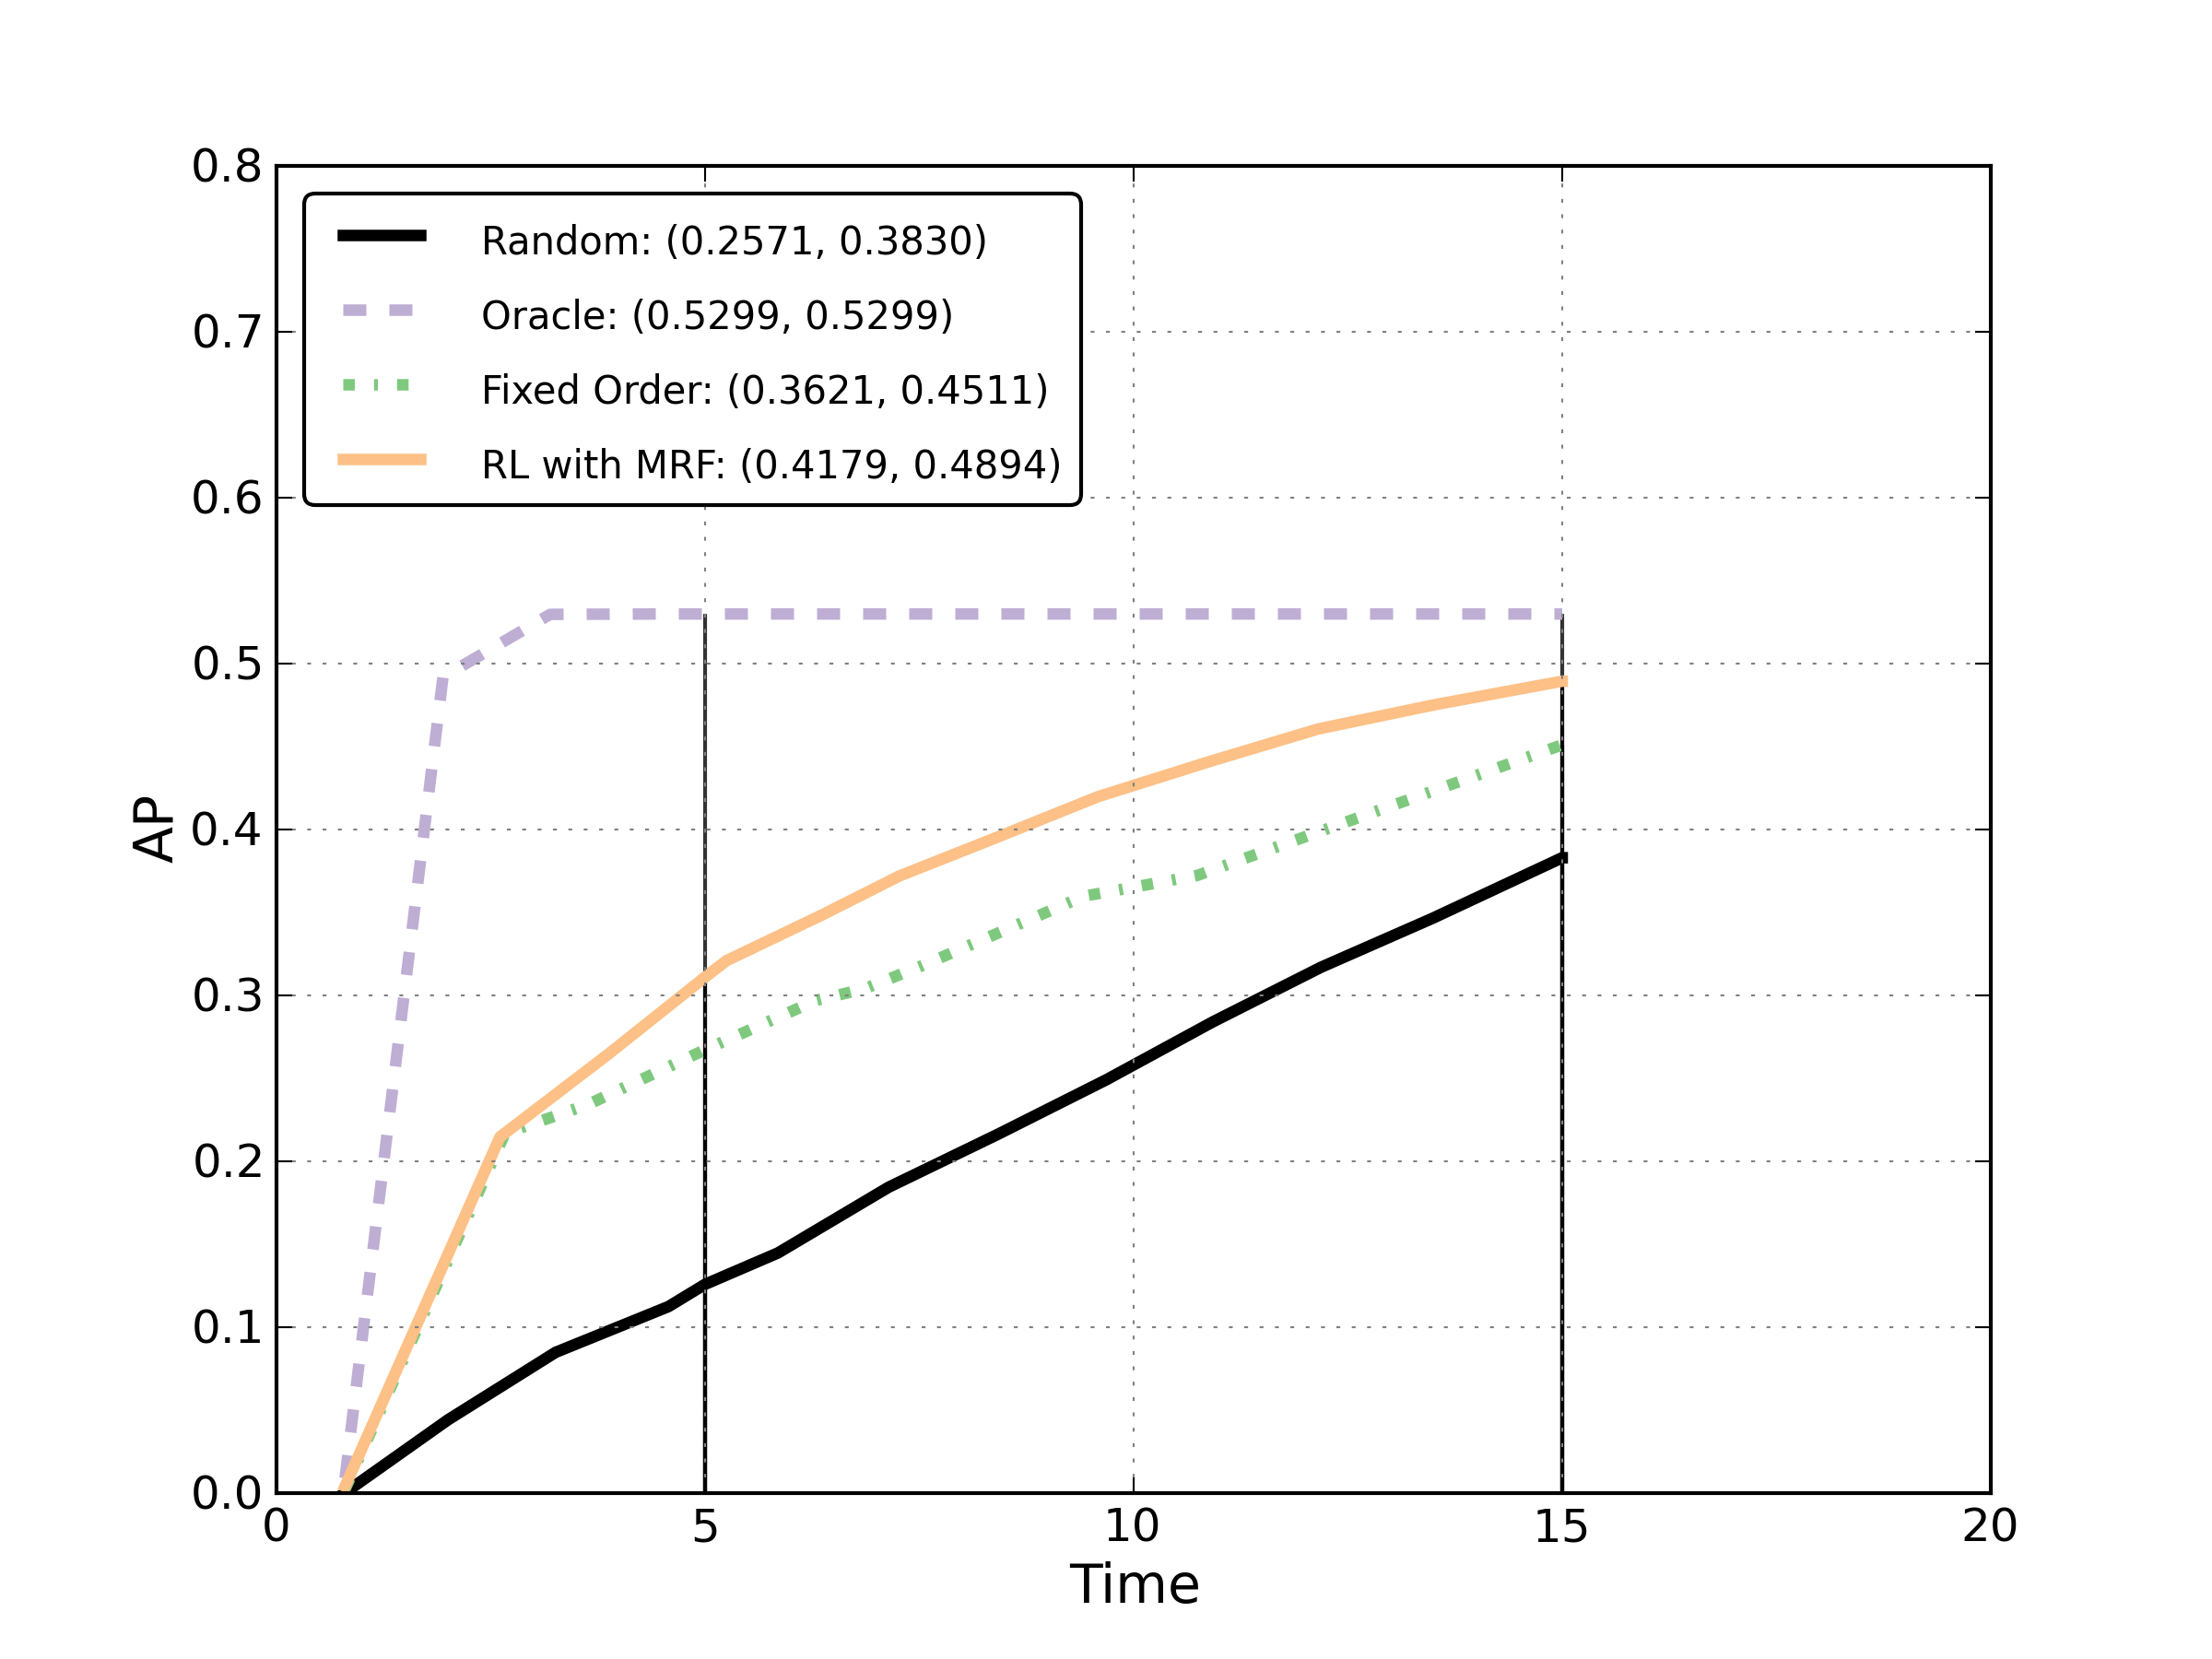
\includegraphics[width=0.47\linewidth]
    {../figures/final1_515.png}\label{fig:results1}} \hfill
\subfloat[]{
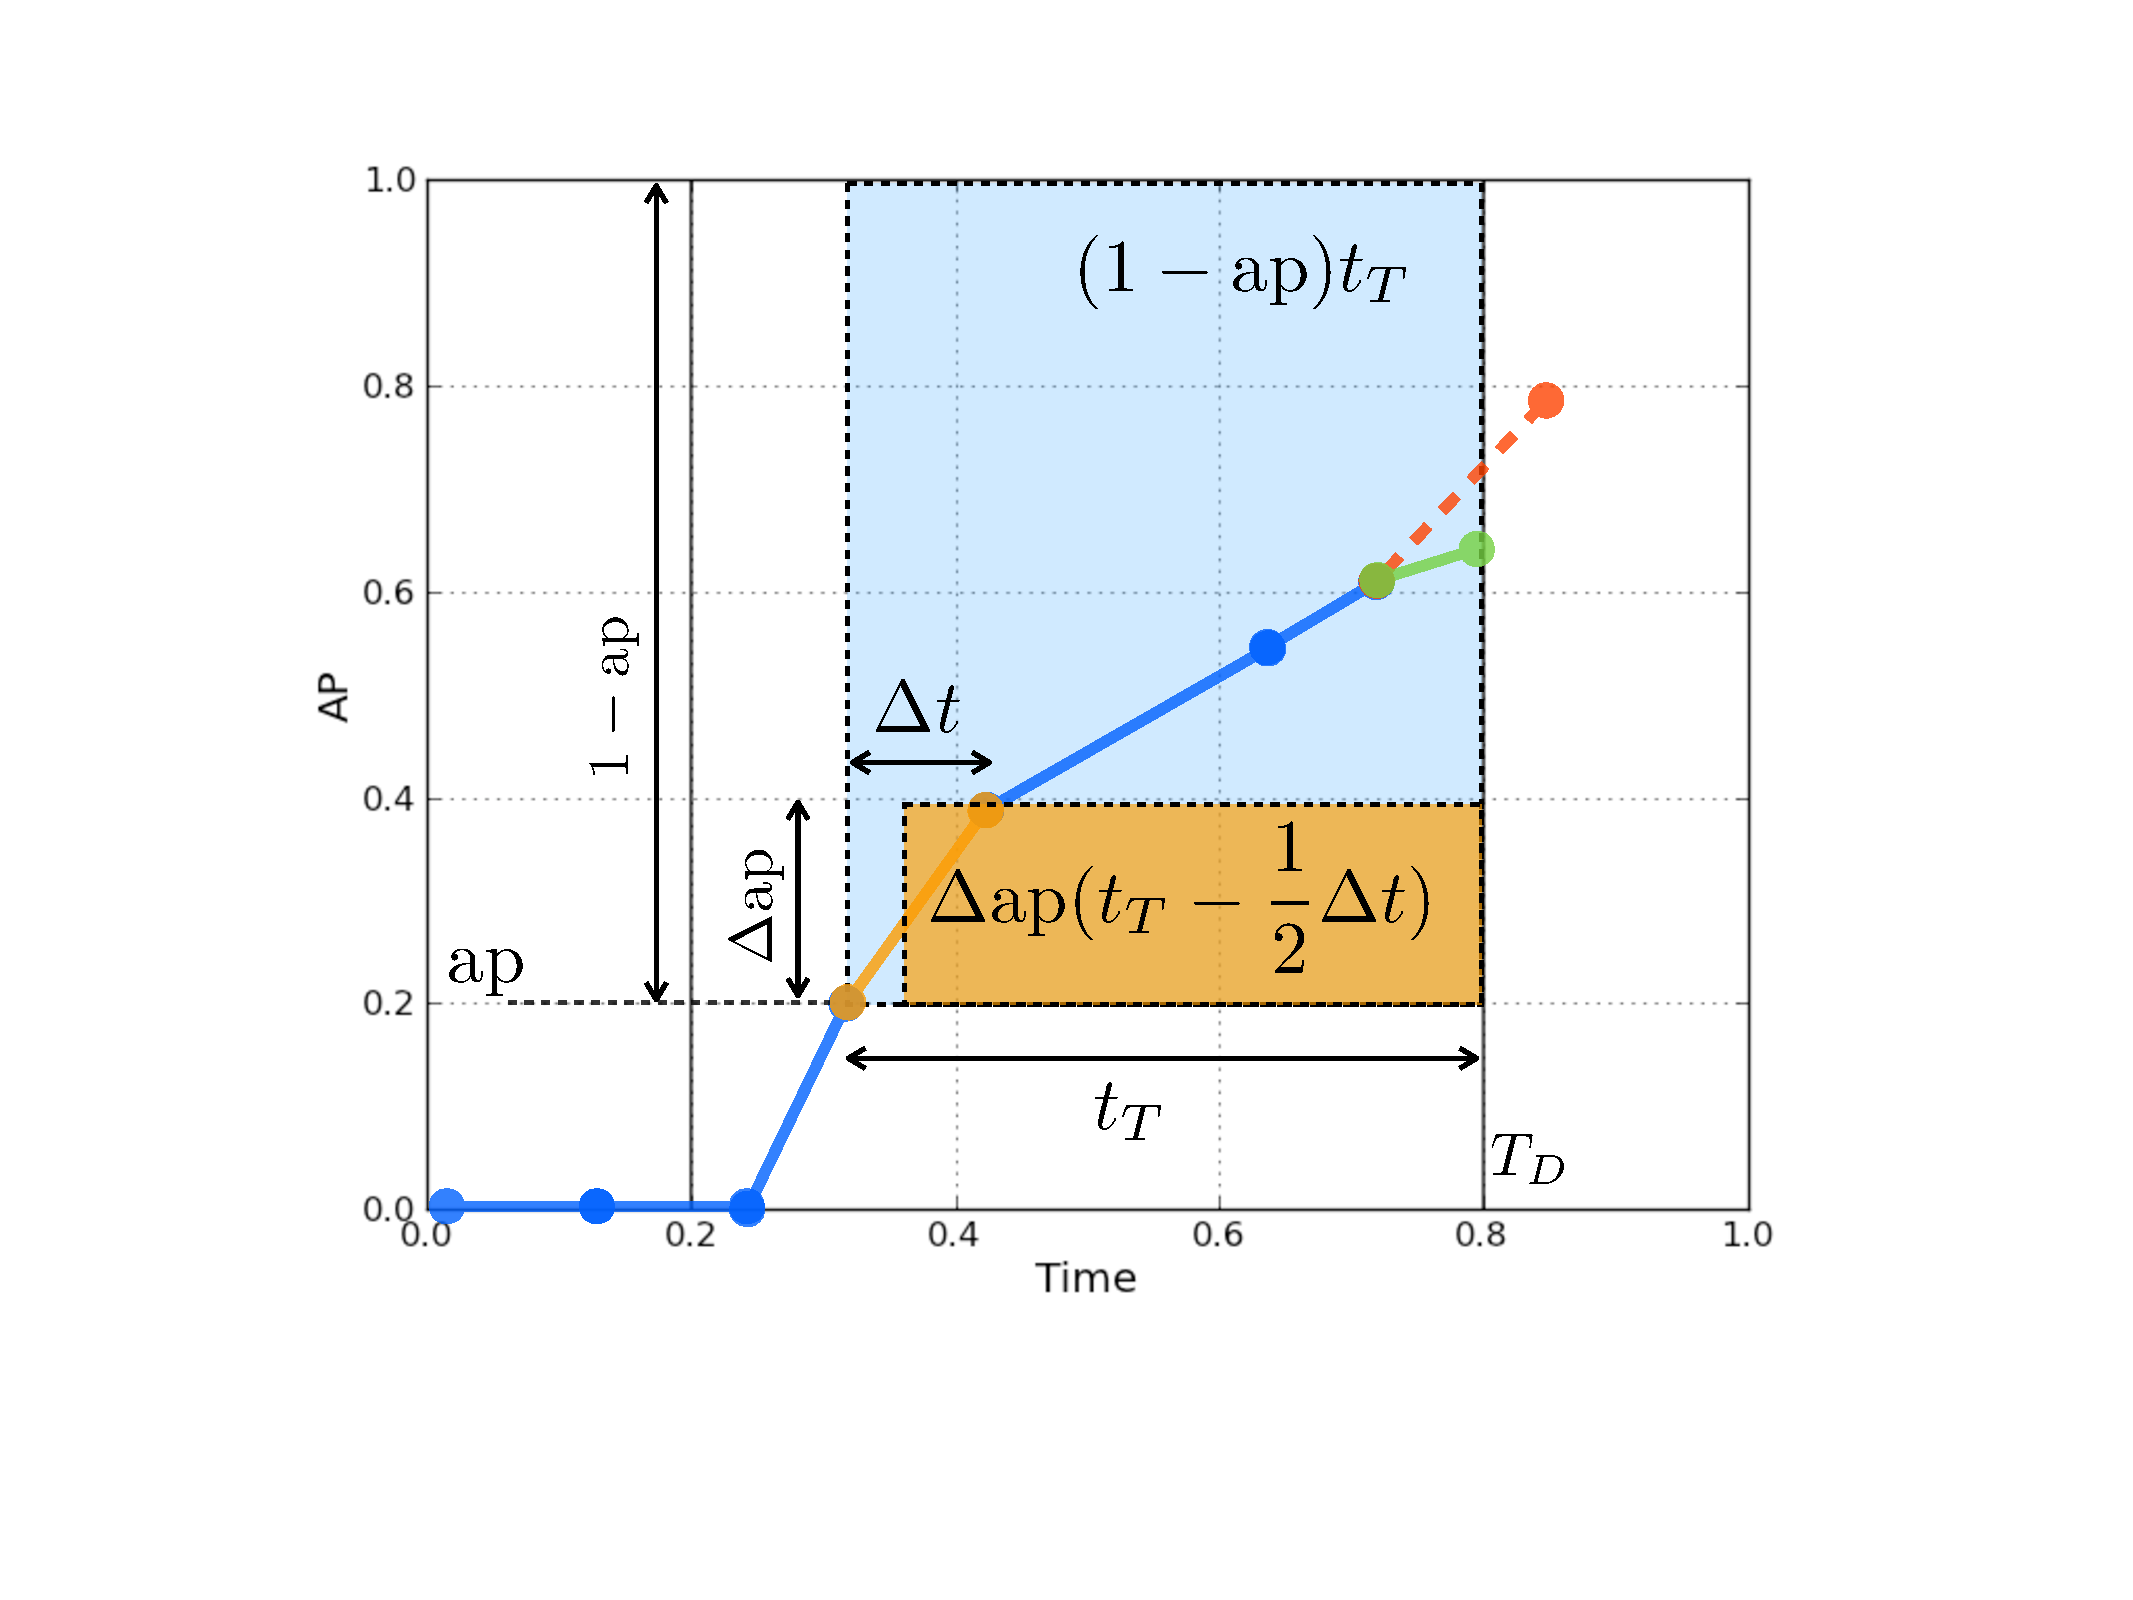
\includegraphics[width=0.47\linewidth]
    {../figures/apvst_expl.pdf}\label{fig:rewards}}
\caption{(a) AP vs. Time curves for Random, Oracle, the Fixed Order baseline, and our best-performing policy, with start time of 5 seconds and deadline of 15 seconds. (b) Reward function explanation.}
\end{figure}

We establish the first baseline for our system by selecting actions randomly at each step.
As shown in Figure \autoref{fig:results1}, this \textbf{Random} policy results in a roughly linear gain of AP vs. time.
This is expected: the detectors are capable of obtaining a certain level of performance; if half the detectors are run, the expected performance level is half of the maximum level.

To establish an upper bound on performance, we plot the \textbf{Oracle} policy, obtained by re-ordering the actions with the hindsight of the results they produced.

We consider another baseline: selecting actions in a fixed order based on the value they bring to the AP vs. Time evaluation, which is roughly proportional to their occurrence probability.
We refer to this as \textbf{Fixed Order}.

Then there are our proposed systems, described in the previous section : \textbf{RL w/ Direct} and \textbf{RL w/ MRF}.
In experiments, the two were not exceedingly different in performance, with the MRF model consistently performing slightly better.

In Figure~\autoref{fig:results1}, we can see that due to the dataset bias, the fixed-order policy performs well at first, as the person class is disproportionately likely to be in the image, but is significantly overtaken by our model as execution goes on and more rare classes have to be detected.

Lastly, we include an additional scene-level GIST feature that updates the posterior probabilities of all classes.
This is considered one action, and takes about $0.3$ seconds.
This setting always uses the MRF model to properly update the class probabilities with GIST observations.
This brings another boost in performance.
All results are shown in \autoref{tab:results}.

\begin{figure}[h!]
  \centering
  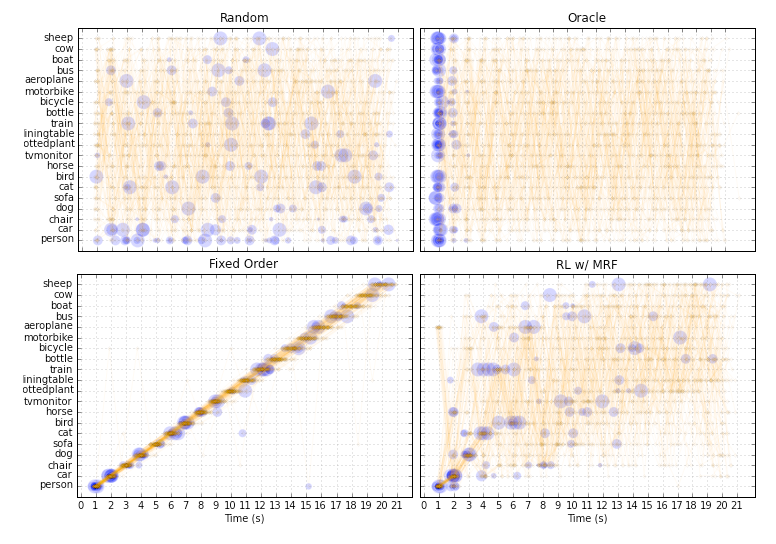
\includegraphics[width=0.86\linewidth]{../figures/trajectories.pdf}
  \caption{
Visualizing the action trajectories of different policies.
Action selection traces are plotted in orange over many episodes; the size of the blue circles correspond to the $\Delta ap$ obtained by the action.
We see that the \textbf{Random} policy selects actions and obtains rewards randomly, while the \textbf{Oracle} policy obtains all rewards in the first few actions.
The \textbf{Fixed Order} policy selects actions in a static optimal order.
Our policy does not stick a static order but selects actions dynamically to maximize the rewards obtained early on.
}
  \label{fig:trajectories}
\end{figure}

Additionally, we evaluated different settings of the discount parameter $\gamma$, and found that a mid-range value works best.
We only report results for that value on the test set.
\autoref{fig:weights} shows how changing $\gamma$ affects the learned weights: the GIST action is learned to never be taken in the greedy setting, because it does not bring any immediate detections results.
In the reinforcement learning setting, however (higher $\gamma$), GIST is learned to be taken for its value in quickly refining the class presence probabilities.

\autoref{fig:trajectories} illustrates the action trajectories of different policies.

\begin{table}[t]
\caption{
The areas under the AP vs. Time curve for different experimental conditions.
Our method reliably beats the intelligent static baseline; including the GIST action further boosts performance.}
\label{tab:results}
\begin{center}
\begin{tabular}{|l|l|l|l|l|l|}
\hline
Bounds & Random & Fixed Order & RL w/ MRF & w/ GIST         & Oracle \\ \hline
(0,20) & 0.250  & 0.342       & 0.378     & \textbf{0.382}  & 0.488 \\ 
(0,10) & 0.119  & 0.240       & 0.266     & \textbf{0.267}  & 0.464 \\ 
(5,15) & 0.257  & 0.362       & 0.418     & \textbf{0.420}  & 0.530 \\ \hline
\end{tabular}
\end{center}
\end{table}
